\documentclass[letterpaper, 10 pt, conference]{ieeeconf}  % Comment this line out if you need a4paper

%\documentclass[a4paper, 10pt, conference]{ieeeconf}      % Use this line for a4 paper

\IEEEoverridecommandlockouts                              % This command is only needed if 
                                                          % you want to use the \thanks command

\overrideIEEEmargins                                      % Needed to meet printer requirements.

% See the \addtolength command later in the file to balance the column lengths
% on the last page of the document

% The following packages can be found on http:\\www.ctan.org
\usepackage{graphicx} % for pdf, bitmapped graphics files
%\usepackage{epsfig} % for postscript graphics files
%\usepackage{mathptmx} % assumes new font selection scheme installed
%\usepackage{times} % assumes new font selection scheme installed
%\usepackage{amsmath} % assumes amsmath package installed
%\usepackage{amssymb}  % assumes amsmath package installed
\usepackage{listings} % allow changing font size for verbatim

\lstset{ %  Set parameters for code listings
language=Python,           % choose the language of the code
numbers=left,           % where to put the line-numbers
numberstyle=\tiny,      % the size of the fonts that are used for the line-numbers
basicstyle=\tiny    % the size of the fonts that are used for the line-numbers
}

\title{\LARGE \bf
Tool for ROS code generation
}

\author{Danying Hu and Yangmin Li and Mohammad Haghighipanah and Blake Hannaford% <-this % stops a space
\thanks{*This work was  supported by NSF Grant xxxxxxxxxxxx  via subcontract from Stanford University}% <-this % stops a space
\thanks{Biorobotics Laboratory, Department of Electrical Engineering, University of Washington, Seattle WA 98195-2500}%
}
\begin{document}



\maketitle
\thispagestyle{empty}
\pagestyle{empty}


%%%%%%%%%%%%%%%%%%%%%%%%%%%%%%%%%%%%%%%%%%%%%%%%%%%%%%%%%%%%%%%%%%%%%%%%%%%%%%%%
\begin{abstract}


(Let's cooperate on this google doc and we can convert to Latex just before submission)

TBD:   Let?s come up with a cool and short name for the tool?. ideas?\\
   ros-helper??\\
   ros\_tool??\\
   ros-o-matic??\\

we can do a global search-replace with  [ros\_tool] $\to$ new-name
 
 \vspace{2.0in}

\end{abstract}


%%%%%%%%%%%%%%%%%%%%%%%%%%%%%%%%%%%%%%%%%%%%%%%%%%%%%%%%%%%%%%%%%%%%%%%%%%%%%%%%
\section{INTRODUCTION}
\subsection{ROS}
ROS\cite{xxxxx} is a widely adopted middleware package for robotics which greatly facilitates cooperation among software modules in a robotic system.   Unfortunately, ROS suffers from a difficult learning curve, especially for programmers who are not well versed in build systems such as CMake.   
ROS has available an excellent set of tutorials\cite{RosTutorialsWWW} which quickly expose the new user to the basic functions.  However, the examples in the tutorials can be hard for new users to generalize into new applications.  Modifying the tutorial examples into desired applications which function independently of the tutorial packages is not straightforward. 

One simple approach to making the learning curve easier is to create template, ``starter", files, which can be customized by the new user.  However, ROS has a large number of capabilities and supports multiple languages.  Thus there are many needed templates.   Specific attributes of ROS nodes which generate different elements in the node code are
\begin{itemize}
  \item Language options: C++ and Python (other languages will not be considered here but ROS support for Java and Lisp exists)
  \item Communication tasks: which can be one or more of Messages, Services, and Actions 
  \item Direction of communication: inbound and outbound communication is referred to by names specific to the task. For example 
  Subscribe and Publish  describe input and output  for messages. 
\end{itemize}

The total number of templates is thus 12 (assuming only one ROS feature is used in the application).  A template-based approach would also require the  user to create build configuration files including ROS and node specific manifest.xml, CMakeLists.txt, and package.xml depending on which of the two ROS build systems (rosbuild  or catkin) will be used.  Counting the two build-system options, the total number of permuations becomes 24!
Many ROS applications (even at the beginner level) require more than one of the above combinations.  For example, a node may publish a message and call a service.  Thus a set of fixed templates is of limited practical use. 
 
For each node which instantiates one or more particular task/language combinations, a ROS application must have
\begin{itemize}
  \item Includes/imports for dependencies
  \item Initialization of the node
  \item Instantiation of classes for task units (message variables, service requests and responses, etc.)
  \item Callbacks (for inbound communications)
  \item Example invocations of some classes (such as {\tt roscpp::publish() or rospy.publish()}) 
  \item Proper argument lists for the class invocations and methods
  \item Correctly configured CMakeLists.txt and package.xml or manifest.xml files. 
\end{itemize}


\section{Approach}
\subsection{Software Description}

ros\_tool assumes that the user has a properly configured ROS workspace already created, that roscore is running, and that a package has been created and initialized in the current workspace.   ros\_tool is written in Python and contains classes which describe and process the ROS package, and a new ROS node, as well as helper functions to explore the package file tree and determine any existing .msg and .srv files.  

The first part of ros\_tool execution collects information from the user about the desired application template including
\begin{itemize}
  \item path to ROS workspace
  \item package name
  \item name of existing messages (.msg) or service (.srv) (if any)
  \item name of existing ros nodes in the package
  \item Desired tasks (Message, Service, or Action) and their directions (e.g. Publish or Subscribe)
\end{itemize}

There are three ways this information is collected.   First, the user can edit a file (param\_node.py) which initializes values for any internal ros\_tool variable.  The  param\_node.py file is executed (via {\tt exec()}) by the main Python script.  The user can thus initialize any value using any valid Python syntax, but basic assignment statements are sufficient for most purposes.  For example, the following lines contained in param\_node.py

\begin{verbatim}
# path to your ROS workspace
rws = '/home/blake/Projects/Ros2/RosNodeGen/'
\end{verbatim}

initialize the variable ``rws" which contains the ROS workspace path. 

A second mode of data collection is to query the user.   This is done with ``rawinput()" statements in the command line.  For example one such input statement prompts the user to enter the name of the node as:

\begin{verbatim}
Enter your new node name: [test_node]: 
\end{verbatim}

The default value, in this case ``test\_node", is accepted if the user hits enter without typing a new value.

Finally, the ros\_tool gets some information by exploring the file system of the selected package.  We use the {\tt rospkg} library (http://www.ros.org/reps/rep-0114.html) to look for msg and service descriptors (.msg and .srv files) which may exist in the package.   Information collected by the three methods is populated into the package and node objects.  

One of the most important user inputs is to specify the language (C++ and Python only in the current version).   Language selection determines the initial template file as well as the templates for the included statements.  As each message or service is fully specified, appropriate statements in the selected language are generated by substituting their data tags and then appended to the section tag statement lists.    After the end of user input, the output files are generated by completing substitution of any remaining data tags and writing the output files. 

\subsection{Generating Output}

ros\_tool uses several template files containing tags which will be filled in with the user's information.    The template files are listed in Table \ref{tagtable}.

\begin{table}\centering
\begin{tabular}{ll}
Filename                                 & Template Target \\ \hline
pyt2\_template.py                   &  Python nodes \\
cpp\_template.cpp                   & C++ nodes \\
CMakeListTemplate.txt        &  CMakeList.txt file \\
MakefileTemplate\\
manifestTemplate.xml \\
msgTemplate.msg              & .msg files \\
srvTemplate.srv                & .srv files\\
\end{tabular}
\caption{Template files used by ros\_tool to generate user node and associated build files.}\label{tagtable}
\end{table}

An example tag is "{\tt \$PKG\$}" which will be replaced by the package name. 

The ros\_tool contains a large number of tag/value pairs which are populated from the node and package classes and used to create the required output files from the templates.   Tags are further divided into two levels, data tags and section tags.   Data tags contain simple values such as the name of a ROS message.  Section tags contain entire sections of generated code such as statements to instantiate several ROS messages to which the application will subscribe  or all the user-specific imports required in a Python node.  Section tags may contain data tags.    

When generating a new node with ros\_tool, the output generates files which are in the right locations and are ready for building with the selected ROS build tool.   All configurations including CMakeList.txt and manifest.xml/package.xml have been automatically updated. Template files for build files are selected based on which of the two build systems are selected.  

Another issue which generates multiple branches in the logic is the potential use of existing message/service/action templates vs. creating custom ones.  As a user prepares an application template, there are several possibilities (although they will be illustrated here with messages they apply to services and actions as well):
\begin{enumerate}
  \item User wishes to use an existing message from another package (e.g. std\_msgs)
  \item User wishes to use a custom message in the current package, .msg file already exists
  \item User wishes to use a custom message in the current package, but has not yet created the .msg file.
\end{enumerate}
ros\_tool supports all three of these cases, prompting the user for necessary information to build a new .msg file if necesssary. 

\section{Example}
In the following example, we create a new Python node in the ``test2" package called ``icra\_2015\_node".  This new node will publish a message (with an existing .msg file in the test2 package) and will call a service (``example\_serv\_2015") as a client.   The user dialog is reproduced in Figure \ref{dialogexample}:

\begin{figure*}
{\small
\begin{verbatim}
Welcome to ROS node generator  *****
Please answer a few questions about your new node:
Enter your package name: test2
start to generate Makefile
Enter your new node name: [test2_node]: icra_2015_node
Enter your language: [Python or C++]: Py
Do you want to add a message? (y for yes, n/CR for no) y
[P]ublish or [S]ubscribe?: Pub
Enter the package that contains your message [test2]
getting path for package: [test2]
Found package path: /home/blake/Projects/Ros2/RosNodeGen/src/test2
Find the following messages in the package /home/blake/Projects/Ros2/RosNodeGen/src/test2/msg/:
1: String.msg
Select message by number: 1
Enter the topic of your message: default [String_topic]icra_2015_tpc
getting path for package: [test2]
Found package path: /home/blake/Projects/Ros2/RosNodeGen/src/test2
this is a comment line
this is a header line
this is an empty line
Do you want to add a message? (y for yes, n/CR for no) 
Do you want to add a service? (y for yes, n/CR for no) y
[C]lient or [S]erver?: Cli
Enter the package that contains your service, default package: [ test2 ]
getting path for package: [test2]
Found package path: /home/blake/Projects/Ros2/RosNodeGen/src/test2
Find the following services in the package /home/blake/Projects/Ros2/RosNodeGen/src/test2/srv/:
1: bh_service.srv
Select service by number: 1
Enter the name of your service: default [bh_service_name]example_serv_2015
getting path for package: [test2]
Found package path: /home/blake/Projects/Ros2/RosNodeGen/src/test2
Do you want to add a service? (y for yes, n/CR for no) 
start to generate the source file for node icra_2015_node in language Python
start to update manifest.xml
start to update CMakeList.txt
\end{verbatim}
}
\caption{Terminal dialog in which ros\_tool creates a node in Python language which can publish to the topic ``icra\_2015\_tpc" and invoke the service ``bh\_service.srv" as a client.}\label{dialogexample}
\end{figure*}

Because this is a Python node, ros\_tool selects  the pyt2\_template.py template file.  The before and after versions of that file are reproduced in Figure \ref{sidebysidecode}.

\begin{figure*}
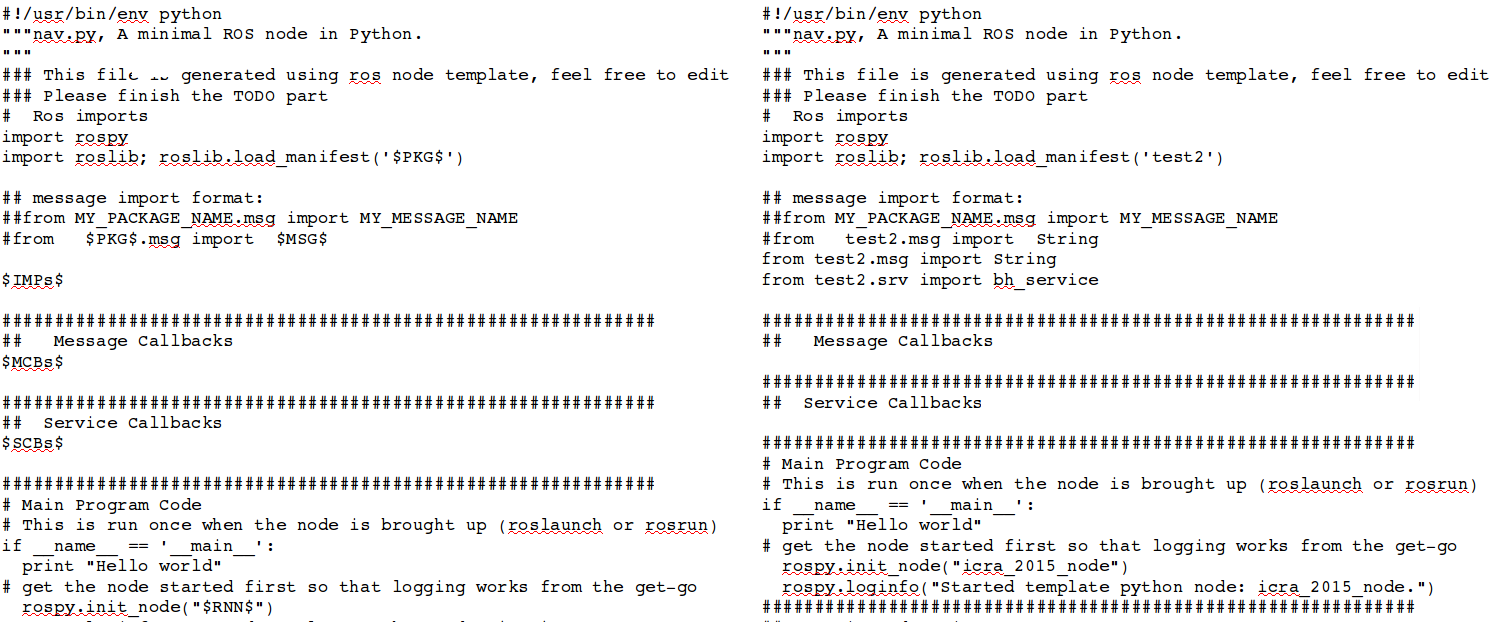
\includegraphics[width=6.25in]{sideBySide1.png}
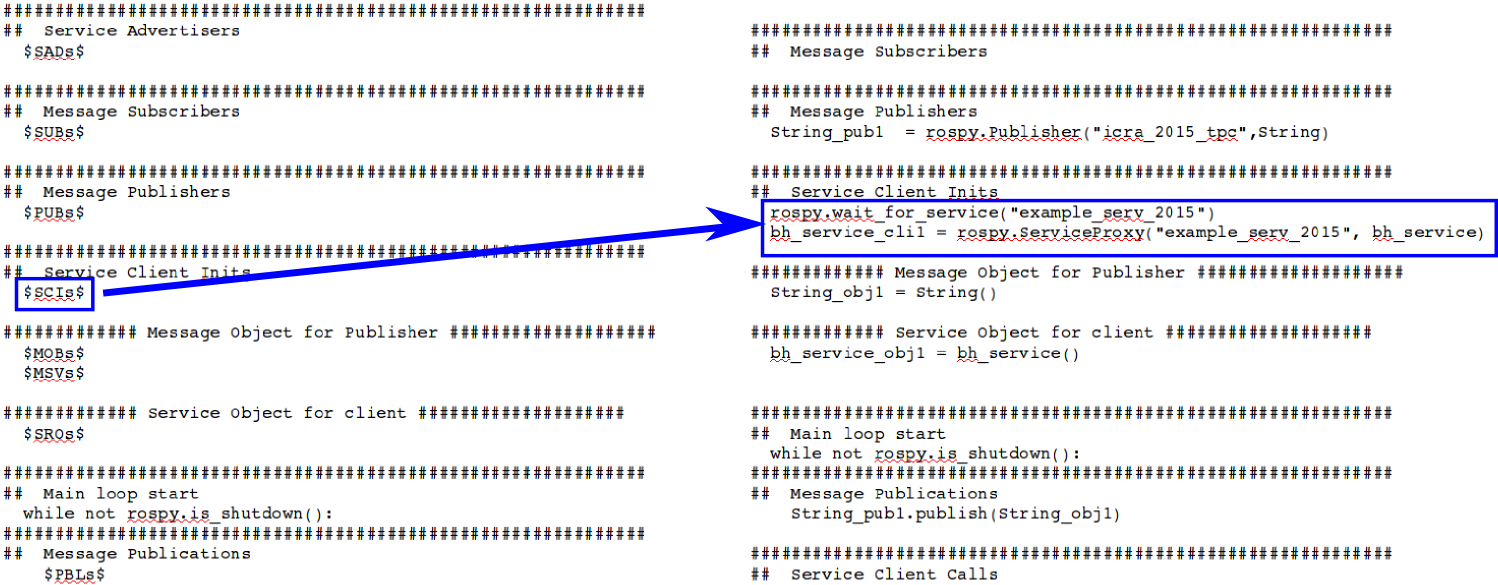
\includegraphics[width=6.25in]{sideBySide2a.png}
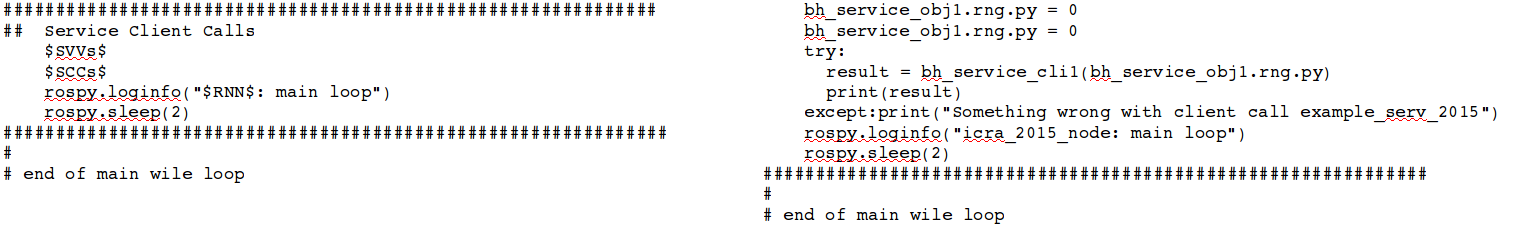
\includegraphics[width=6.25in]{sideBySide3.png}
\caption{Python template file (left) and completed node file (right). Boxes and arrows illustrate one case of tag substitution.}
\label{sidebysidecode}
\end{figure*}

\section{Discussion and Future Work}
The contribution of this work is a new software package to streamline the process of creating a new ROS node for robotics control. 
The package automatically generates 
code for a new node source file in either C++ or Python.  It also creates
build-configuration files for either rosbuild or catkin build systems and 
.msg or .srv files if necessary

ros\_tool source code and template files are available on github: *****URL******
\subsection{Limitations}
As with all software, the ros\_tool has limitations:
Much of the user input is based on a clunky command line interface.  GUI support (through a package like tkinter/ttk) should be implemented.
Python indentation needs adjustment by the user and should be automatically corrected as tags are filled in with values.
Configuration files such as CMakeLists.txt are created from the generic template files and so if a package contains existing nodes, the old CMakeLists.txt file must be saved and manually merged with the new one. 
Variable names for new custom messages and services are auto-generated and thus not descriptive for the applications semantics.  

\subsection{Future Work }
Our current priorities for future improvements to ros\_tool are
\begin{itemize}
 \item Generate correct indentation on Python output
 \item Extend functionality to ROS actions
 \item Adapt the build-file output system to modify existing CMakeList.txt instead of creating from scratch.
\end{itemize}

The ros\_tool code is open source (LGPL) and we encourage users to identify and fix bugs and limitations to ros\_tool and participate in a community effort to simplify ROS development. 
\end{document}
